\chapter{THIẾT KẾ BỘ ĐIỀU KHIỂN CTC (Computed-Torque Control)}
    \section{Tiêu chí thiết kế}
    \hspace*{0.6cm}Tiêu chí thiết kế:
    \begin{itemize}
        \item Settling time: $T_s < 4\text{s}$
        \item Overshoot: \%OS < 10\%
    \end{itemize}

    Đối với hệ thống bậc 2, ta có:

    \[
    T_s = \frac{4}{\omega_n}, \quad \%OS = 100e^{\left(-\zeta\pi / \sqrt{1-\zeta^2}\right)}
    \]

    Hệ số giảm chấn $\zeta$ tính từ \%OS:

    \[
    \zeta = \frac{-\ln\left(\frac{\%OS}{100}\right)}{\sqrt{\pi^2 + \ln^2\left(\frac{\%OS}{100}\right)}} = 0.5911
    \]

    Chọn $\zeta = 0.7$

    Suy ra:

    \[
    \omega_n > \frac{4}{\zeta T_s} = \frac{4}{0.7 \cdot 4} = 1.42857
    \]

    Chọn $\omega_n = 1.5 \text{ (rad/s)}$

    \section{Computed-Torque Control}
            Từ hệ phương trình (1.16), ta đưa về dạng tổng quát
            \begin{equation}
                M(q) \ddot{q} + C (q, \dot{q}) \dot{q} + G(q) = \tau
            \end{equation}
            Trong đó
            \begin{itemize}
                \item $q = [x \,\, \theta]^T$: vector trạng thái
                \item $M(q)$: ma trận quán tính
                \item $C(q, \dot{q})$: ma trận Coriolis và ly tâm
                \item $G(q)$: vector trọng lực
                \item $\tau$: moment xoắn điều khiển từ động cơ
            \end{itemize} 
            Ta được
            \begin{align*}
                &\underbrace{
                \begin{bmatrix}
                M_\Sigma & M_p \ell \cos \theta\\
                M_p \ell  \cos \theta & J
                \end{bmatrix}
                }_{M(q)}
                \begin{bmatrix}
                \ddot{x} \\ \ddot{\theta}
                \end{bmatrix}
                +
                \underbrace{
                \begin{bmatrix}
                0 & -M_p \ell \dot{\theta} \sin \theta \\
                0 & 0
                \end{bmatrix}
                }_{C(q, \dot{q})}
                \begin{bmatrix}
                \dot{x} \\ \dot{\theta}
                \end{bmatrix} 
                +
                \underbrace{
                \begin{bmatrix}
                0 & 0 \\
                0 & -M_p g \ell \sin \theta
                \end{bmatrix}
                }_{G(q)}
                =
                \underbrace{
                \begin{bmatrix}
                F_x \\
                \tau
                \end{bmatrix}
                }
            \end{align*}
        Định nghĩa lỗi theo dõi
        \begin{align}
            &e(t) = q_d(t) - q(t) \nonumber \\
            &\dot{e}(t) = \dot{q}_d(t) - \dot{q}(t) \nonumber \\
            &\ddot{e}(t) = \ddot{q}_d(t) - \ddot{q}(t) \nonumber
        \end{align}
        Ta có thể viết lại
        \begin{align}
            \ddot{e} = \ddot{q}_d(t) + M^{-1} (C(q, \dot{q})\dot{q} + G(q) - \tau)  \nonumber
        \end{align}
        Đặt tín hiệu điều khiển $u$ trở thành
        \begin{align}
            u = \ddot{q}_d(t) + M^{-1} (C(q, \dot{q})\dot{q} + G(q) - \tau)  
        \end{align}
        Ở đây giả sử cho nhiễu môi trường 
        \begin{align*}
            \tau_d = 0
        \end{align*}
        Khi đó 
        \begin{align*}
            \ddot{e} = u
        \end{align*}
        Từ phương trình (2.1), moment xoắn đầu ra được tính như sau
        \begin{align}
            \tau = M(q)(\ddot{q_d} - u) + C(q, \dot{q})\dot{q} + G(q)
        \end{align}         
        Giả sử chọn $u$ như là một bộ điều khiển PD, ta có
        \begin{align*}
            u = - K_p e - K_d \dot{e}
        \end{align*}
        Với $K_p$ và $K_d$ là ma trận điều khiển tỉ lệ và vi phân tương ứng. Khi đó phương trình (2.3) trở thành
        \begin{align}
            \tau = M(q)(\ddot{q_d} + K_p e + K_d \dot{e}) + C(q, \dot{q})\dot{q} + G(q)
        \end{align} 
        Phương trình vòng kín của lỗi động lực học
        \begin{align}
            \ddot{e} + K_p e + K_d \dot{e} = 0
        \end{align}
        Trong không gian trạng thái
        \begin{align*}
            \frac{d}{dt}
            \begin{bmatrix}
            e \\ \dot{e}
            \end{bmatrix}
            =
            \begin{bmatrix}
            0 & I \\
            -K_p & -K_d
            \end{bmatrix}
            \begin{bmatrix}
            e \\ \dot{e}
            \end{bmatrix}
        \end{align*}
        Phương trình đặc trưng
        \begin{align*}
            s^2 + K_d s + K_p = 0
        \end{align*}
        Có dạng chuẩn theo yêu cầu thiết kế
        \begin{align*}
            s^2 + 2\zeta \omega_n s + \omega_n^2 = 0
        \end{align*}
        So sánh ta thu được
        \begin{equation*}
            \begin{cases}
                K_d = 2\zeta \omega_n  = 2 \cdot 0.7 \cdot 1.5 = 2.1\\
                K_p = \omega_n^2 = 1.5^2 = 2.25
            \end{cases}
        \end{equation*}
        Đồ thị đáp ứng của vị trí góc (ban đầu góc $-\dfrac{\pi}{2}$, tức là ban đầu xe nằm ngang)
        \begin{figure}[H]
            \centering
            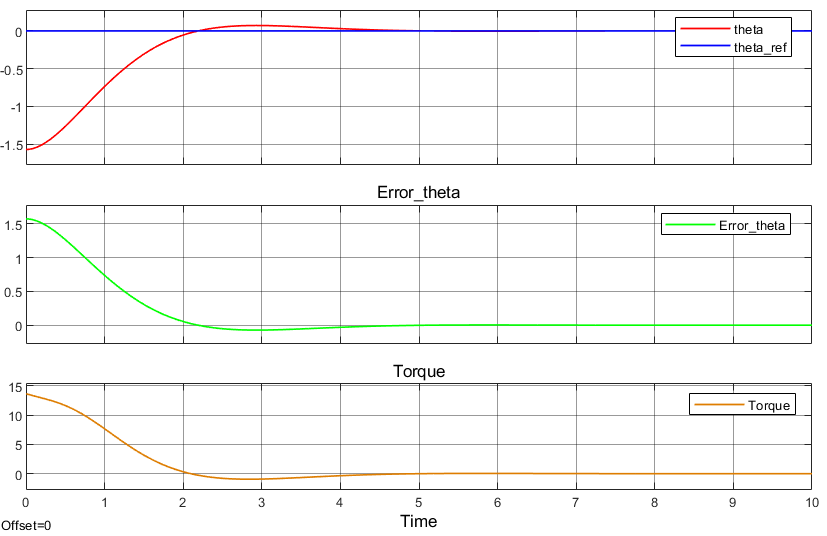
\includegraphics[width=1\textwidth]{pictures/torce.png}
            \caption{Đáp ứng vị trí góc}
        \end{figure}
        Đồ thị đáp ứng của vị trí
        \begin{figure}[H]
            \centering
            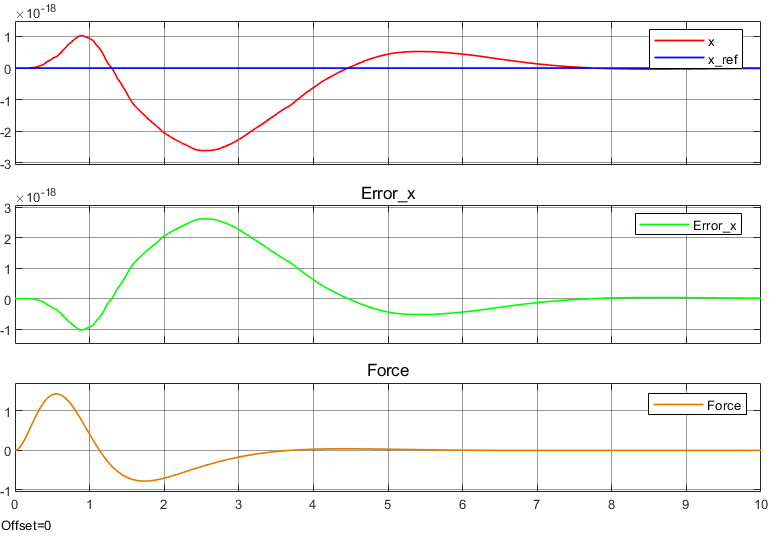
\includegraphics[width=1\textwidth]{pictures/force.png}
            \caption{Đáp ứng vị trí}
        \end{figure}